\documentclass{scirep}
\usepackage[T1]{fontenc}
\usepackage{chemformula}
\usepackage{graphicx}
\usepackage{amsmath}

\leftheader{Studium atomových emisních spekter}
\centerheader{Praktikum IV}
\rightheader{Tomáš Derner}

\begin{document}

    \section*{Úkol}

    \begin{enumerate}

        \item S použitím spektra rtuti zkalibrujte hranolový spektrometr.
        Pro vyloučení hrubých chyb vyneste kalibrační křivku ihned do grafu.
        \item Ověřte vlnové délky sodíkových dubletů (alespoň tří).
        \item Na základě pozorování sodíkových dubletů diskutujte rozlišovací schopnost spektrometru.
        Diskutujte přesnost takto určené rozlišovací schopnosti.
        \item Prohlédněte si spektra výbojek s náplní \ch{He}, \ch{Ne}, \ch{Ar}, \ch{N2} a \ch{CO2}.
        Určete vlnové délky nejjasnějších čar.
        Porovnejte s tabulkovými hodnotami.
        \item Změřte vlnové délky čar \ch{H_{$\alpha$}}, \ch{H_{$\beta$}}, \ch{H_{$\gamma$}} Balmerovy serie vodíkového spektra.
        Vypočítejte Rydbergovu konstantu.

    \end{enumerate}

    \section*{Teorie}

    V této úloze studujeme atomová emisní spektra plynů.
    Využíváme k tomu hranolový spektrometr Hilgerova typu, jehož detailní popis je uveden ve studijním textu~\cite{pokyny}.
    Tento spektrometr neudává přímo vlnové délky pozorovaných čar, je proto potřeba jej okalibrovat pomocí známých vlnových délek emisního spektra rtuti.
    Tabulkové hodnoty těchto vlnových délek jsou uvedeny v sekci výsledků měření v tabulce~\ref{tab:calibration}.

    Pro rozlišovací schopnost $r$ spektrometru platí vztah
    \begin{equation}
        \label{eq:R}
        r = \frac{\lambda}{d\lambda},
    \end{equation}
    který určuje minimální rozdíl vlnových délek $\lambda$ a $\lambda + d\lambda$, který ještě spektrometr dokáže rozlišit.
    V tomto případě využijeme pro určení rozlišovací schopnosti měření dubletů sodíku.

    Ve viditelném emisním spektru vodíku jsou pozorovatelné čtyři čáry \ch{H_{$\alpha$}} (červená), \ch{H_{$\beta$}} (modrozelená), \ch{H_{$\gamma$}} (modrá) a \ch{H_{$\delta$}} (fialová).
    Tyto čáry jsou součástí tzv. Balmerovy série, pro vlnočty jejíž spektrálních čár platí vztah
    \begin{equation}
        \label{eq:rydberg}
        \sigma = \frac{1}{\lambda} = R \left( \frac{1}{4} - \frac{1}{n^2} \right),
    \end{equation}
    kde $R$ je Rydbergova konstanta a $n = 3, 4, 5, 6$ jsou přirozená čísla odpovídající jednotlivým čarám.
    Rydbergovu konstantu určíme z tohoto vztahu metodou nejmenších čtverců.



    \section*{Výsledky}

    \subsection*{Úkol 1}

    Pomocí tabulkových hodnot vlnových délek spektrálních čar rtuti byla provedena kalibrace hranolového spektrometru.
    Skutečné hodnoty a naměřené hodnoty v obecných jednotkách jsou uvedeny v tabulce~\ref{tab:calibration} a vzniklá kalibrační křivka je zobrazena v grafu na obrázku~\ref{fig:u1}.
    Pro fit kalibrační křivky byl použit polynom pátého řádu, $f(x) = ax^5 + bx^4 + cx^3 + dx^2 + ex + f$, jehož koeficieny $a$ až $f$ jsou uvedeny v tabulce~\ref{tab:parameters}.

    \begin{table}[b]
        \centering
        \setlength{\tabcolsep}{15pt}
        \begin{tabular}[t]{
S[table-format=3.1]
S[table-format=4.0]
}
    \toprule
    {$\lambda$} & {hodnota na stupnici} \\
    {[nm]} & {[obecné jednotky]}  \\ \midrule
690.7	& 3285 \\
671.6	& 3226 \\
623.4	& 3055 \\
612.3	& 3009 \\
607.3	& 2986 \\
579.1	& 2852 \\
577.0	& 2841 \\
546.1	& 2663 \\
491.6	& 2244 \\
435.8	& 1582 \\
434.8	& 1567 \\
433.9	& 1552 \\
407.8	& 1095 \\
404.7	& 1030 \\
 \bottomrule
\end{tabular}
        \caption{Tabulkové hodnoty vlnových délek spektrálních čar rtuti a naměřené hodnoty v obecných jednotkách spektrometru}
        \label{tab:calibration}
    \end{table}

    \begin{table}[b]
        \centering
        \setlength{\tabcolsep}{15pt}
        \begin{tabular}[t]{
c
S[table-format=2.2e2]
S[table-format=1.2e2]
}
    \toprule
    {parametr} & {hodnota} & {chyba}    \\ \midrule
a &	5.36e-15	&   0.93e-16    \\
b &	-4.81e-11   &  	1.03e-11    \\
c &	1.80e-07	&   0.45e-08    \\
d &	-3.18e-04   &  	0.92e-05    \\
e &	3.18e-01	&   0.92e-02    \\
f &	2.66e+02	&   0.34e+01    \\
 \bottomrule
\end{tabular}
        \caption{Parametry fitu kalibrační křivky}
        \label{tab:parameters}
    \end{table}

    \begin{figure}[b]
        \centering
        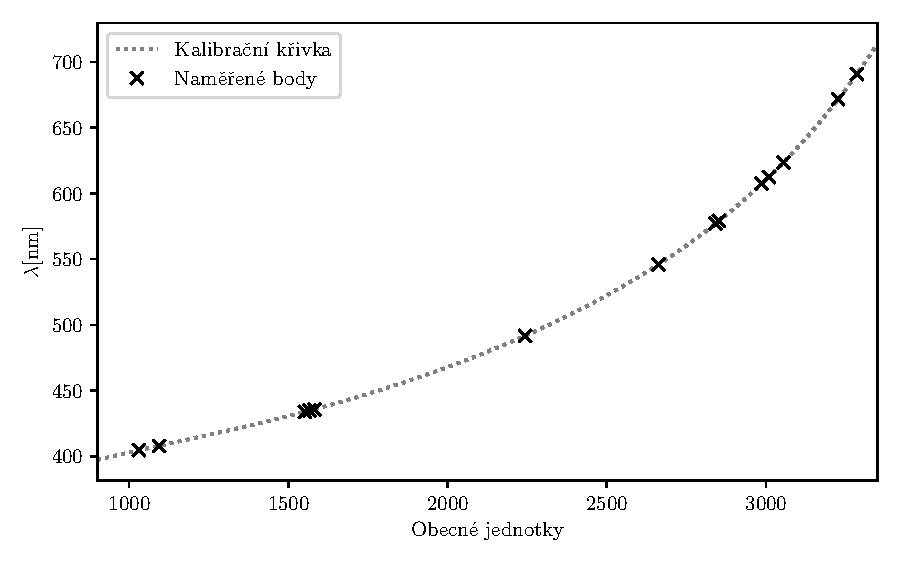
\includegraphics{u1.pdf}
        \caption{Kalibrační křivka pro použitý spektrometr}
        \label{fig:u1}
    \end{figure}

    \subsection*{Úkol 2 a 3}
    V tabulce~\ref{tab:doublets} jsou uvedené tabulkové hodnoty vlnových délek sodíkových dubletů $\lambda_{tab}$ a naměřené hodnoty téhož $\lambda_m$.
    Tyto hodnoty jsou pak doplněny rozdíly vzdáleností obou čar v daném dubletu $d\lambda_{tab}$ resp. $d\lambda_m$.
    Poslední sloupec pak obsahuje rozdíl tabulkové a naměřené hodnoty pro tyto spektrální čáry.
    Soudě podle čtvrtého uvedeného dubletu v tabulce není rozlišovací schopnost spektrometru definovaná vztahem~\eqref{eq:R} lepší než \SI{e3}{}.

    \begin{table}[b]
        \centering
        \setlength{\tabcolsep}{15pt}
        \begin{tabular}[t]{
S[table-format=3.1]
S[table-format=1.1]
S[table-format=4.0]
S[table-format=3.1]
S[table-format=1.1]
S[table-format=1.1]
}
    \toprule
    {$\lambda_{tab}$} & {$d\lambda_{tab}$} & {hodnota na stupnici} & {$\lambda_m$} & {$d\lambda_m$} & {$\left\| \lambda_{tab} - \lambda_m \right\|$} \\
    {[nm]} & {[nm]} & {[obecné jednotky]} & {[nm]} & {[nm]} & {[nm]}  \\ \midrule
616.1	&   0.7     &   3022    &   615.6   &   0.3   & 0.5  \\
615.4	&           &   3021    &   615.3   &         & 0.1  \\ \midrule[0pt]
589.6	&   0.6	    &   2903    &   589.2   &   0.4   & 0.4  \\
589.0	&           &   2901    &   588.8   &         & 0.2  \\ \midrule[0pt]
568.9	&   0.1     &   2796    &   568.5   &   0.4   & 0.4  \\
568.8	&           &   2794    &   568.1   &         & 0.7  \\ \midrule[0pt]
515.4	&   0.5     &   2442    &   514.9   &   0.0   & 0.5  \\
514.9	&           &   2442    &   514.9   &         & 0.0  \\ \midrule[0pt]
498.3	&   0.4     &   2302    &   498.1   &   0.1   & 0.2  \\
497.9	&           &   2301    &   498.0   &         & 0.1  \\
 \bottomrule
\end{tabular}

        \caption{Tabulkové a naměřené hodnoty vlnových délek dubletů sodíku a jejich rozdíly}
        \label{tab:doublets}
    \end{table}

    \subsection*{Úkol 4}
    Tabulka~\ref{tab:lines} obsahuje naměřené hodnoty vlnových délek spektrálních čar různých plynů.

    \begin{table}[b]
        \centering
        \setlength{\tabcolsep}{9pt}
        \begin{tabular}[t]{
S[table-format=4.0]
S[table-format=3.1]
S[table-format=4.0]
S[table-format=3.1]
S[table-format=4.0]
S[table-format=3.1]
S[table-format=4.0]
S[table-format=3.1]
S[table-format=4.0]
S[table-format=3.1]
}
    \toprule
    {Ar}        &   {$\lambda_{\text{Ar}}$} &   {He}        &   {$\lambda_{\text{He}}$} &  {Ne}     &   {$\lambda_{\text{Ne}}$}	&   {CO\textsubscript{2}}   &   {$\lambda_{\text{CO\textsubscript{2}}}$}   &   {N}         &   {$\lambda_{\text{N}}$}  \\
    {[o. j.]}   &   {[nm]}                  &   {[o. j.]}   &   {[nm]}                  & {[o. j.]} &   {[nm]}                  &   {[o. j.]}               &   {[nm]}                                     &   {[o. j.]}   &   {[nm]}                  \\ \midrule
    3439        &   749.2	                &	3216        &   668.3     	            &	3322	&   703.6     	            &   2988  	                &   607.6     	                               &   3218  	    &   669.0                  \\
    2971        &   603.8	                &	3024        &   616.0     	            &	3122	&   641.1     	            &   2754  	                &   561.1     	                               &   3190  	    &   660.5                  \\
    2794        &   568.1	                &	2897        &   588.0     	            &	3018	&   614.6     	            &   2480  	                &   519.8     	                               &   3165  	    &   653.1                  \\
    2475        &   519.1	                &	2578        &   533.2     	            &	2886	&   585.7     	            &   2164  	                &   483.4     	                               &   2986  	    &   607.2                  \\
    2030        &   470.5	                &	2334        &   501.8     	            &	2625	&   540.2     	            &   1789  	                &   450.4     	                               &   2836  	    &   575.9                  \\
    1798        &   451.1	                &	2251        &   492.5     	            &	1605	&   437.3     	            &   1625  	                &   438.6     	                               &   2605  	    &   537.2                  \\
    1324        &   420.3	                &	2040        &   471.4     	            &	2037	&   471.2     	            &   1180  	                &   412.5     	                               &   2144  	    &   481.4                  \\
    2690        &   550.3	                &	1744        &   447.0     	            &	2354	&   504.1     	            &   3198  	                &   662.9     	                               &   1874  	    &   457.1                  \\
    2918        &   592.3	                &	       	    &      	                    &       	&      	                    &      	                    &      	                                       &   1441  	    &   427.0                  \\
    3306        &   698.0                   &	       	    &      	                    &       	&      	                    &      	                    &      	                                       &      	        &                          \\
 \bottomrule
\end{tabular}

        \caption{Naměřené hodnoty vlnových délek spektrálních čar různých plynů}
        \label{tab:lines}
    \end{table}

    \subsection*{Úkol 5}

    V tabulce~\ref{tab:h} jsou uvedeny tabulkové a naměřené hodnoty vlnových délek spektrálních čar $\alpha$, $\beta$ a $\gamma$ vodíku a odpovídající hodnoty $n$ ve vztahu~\eqref{eq:rydberg}.
    Pomocí lineární regrese zobrazené v grafu na obrázku~\ref{fig:rydberg} získáme Rydbergovu konstantu
    \[ R = \SI{10965 \pm 17 e3}{\per\metre}. \]
    Tabulková hodnota Rydbergovy konstanty je
    \[ R_{tab} = \SI{10973.732 e3}{\per\metre}. \]

    \begin{table}[b]
        \centering
        \setlength{\tabcolsep}{15pt}
        \begin{tabular}[t]{
S[table-format=4.0]
S[table-format=3.1]
S[table-format=3.1]
S[table-format=1.0]
}
    \toprule
    {hodnota na stupnici} & {$\lambda_{m}$} & {$\lambda_{tab}$} & {$n$} \\
    {[obecné jednotky]}   & {[nm]}          & {[nm]}            & {[]}  \\ \midrule
    3178                  & 656.9           & 656.3             & 3     \\
    2193                  & 486.4           & 486.1             & 4     \\
    1558                  & 434.2           & 434.0             & 5     \\
 \bottomrule
\end{tabular}
        \caption{Tabulkové a naměřené hodnoty vlnových délek spektrálních čar vodíku a odpovídající $n$}
        \label{tab:h}
    \end{table}

    \begin{figure}[b]
        \centering
        \includegraphics{rydberg.pdf}
        \caption{Lineární regrese naměřených vlnových délek čar vodíku}
        \label{fig:rydberg}
    \end{figure}

    \section*{Diskuse}

    Fit kalibrační křivky proveden bezprostředně po naměření hodnot vlnových délek spektrálních čar rtuti umožnil průběžně kontrolovat naměřené hodnoty čar ostatních zdrojů s tabulkovými hodnotami a tak se vyhnout hrubé chybě.
    Určitá chyba kalibrace byla způsobena jednak omezenou přesností spektrometru, tak i faktem, že především v modré oblasti spektra značně záleželo na úhlu, pod kterým se pozorovatel díval do okuláru.

    Rozlišovací schopnost spektrometru byla určena na $\SI{e3}{}$, avšak tato hodnota je značně spekulativní.
    Je pravda, že v jednom případě se dublet, jehož čáry mají podle tabulek vzdálenost $\SI{0.5}{nm}$, nepodařilo rozlišit, naopak se až podezřele dobře podařilo rozlišit dublet se vzdáleností pouze $\SI{0.1}{nm}$, který měl navíc ještě vyšší vlnovou délku.

    Rydbergovu konstantu se podařilo určit v rámci chyby shodně s tabulkovou hodnotou.



    \section*{Závěr}

    Hranolový spektrometr byl úspěšně zkalibrován, byly proměřeny hodnoty vlnových délek sodíkových dubletů a pomocí tohoto měření byla odhadnuta rozlišovací schopnost spektrometru
    \[r = \SI{e3}{}.\]
    Dále byly určeny vlnové délky nejjasnějších čar několika plynových vzorků včetně vodíku, z jehož čar byla spočítána Rydbergova konstanta
    \[ R = \SI{10965 \pm 17 e3}{\per\metre}. \]

    \begin{thebibliography}{}

        \bibitem{pokyny}
        Pokyny k měření ``Studium atomových spekter'', dostupné z\\ \url{https://physics.mff.cuni.cz/vyuka/zfp/_media/zadani/texty/txt_415.pdf}, 12.\,11.\,2019

    \end{thebibliography}

\end{document}